\documentclass{article}   

\usepackage{geometry}
\usepackage{qtree}
\usepackage[square,numbers]{natbib}
% \usepackage{cite}  
\geometry{a4paper}

\usepackage[utf8]{inputenc}
\usepackage[T1]{fontenc}    % use 8-bit T1 fonts
\usepackage{lmodern}
\usepackage{hyperref}       % hyperlinks
\usepackage{lipsum}

\usepackage[protrusion=true,expansion=true]{microtype}

\usepackage{amssymb}
\usepackage{amsfonts}
\usepackage{eqnarray,amsmath}
\usepackage[table]{xcolor}

\usepackage{listings}
\usepackage{graphicx}
\usepackage{dirtytalk}

\usepackage[table]{xcolor}
\usepackage{rotating}
\usepackage{caption}

%% if you use PostScript figures in your article
%% use the graphics package for simple commands
\usepackage{graphics}


%% or use the graphicx package for more complicated commands
\usepackage{graphicx}
\usepackage[table]{xcolor}

\usepackage{indentfirst}
\usepackage[utf8]{inputenc}
 
\usepackage{listings}
\usepackage{xcolor}
 
\definecolor{codegreen}{rgb}{0,0.6,0}
\definecolor{codegray}{rgb}{0.5,0.5,0.5}
\definecolor{codepurple}{rgb}{0.58,0,0.82}
\definecolor{backcolour}{rgb}{0.95,0.95,0.92}
 
\lstdefinestyle{mystyle}{
    backgroundcolor=\color{backcolour},   
    commentstyle=\color{codegreen},
    keywordstyle=\color{magenta},
    numberstyle=\tiny\color{codegray},
    stringstyle=\color{codepurple},
    basicstyle=\ttfamily\footnotesize,
    breakatwhitespace=false,         
    breaklines=true,                 
    captionpos=b,                    
    keepspaces=true,                 
    numbers=left,                    
    numbersep=5pt,                  
    showspaces=false,                
    showstringspaces=false,
    showtabs=false,                  
    tabsize=2
}
 
\lstset{style=mystyle}
% please place your own definitions here and don't use \def but
% \newcommand{}{}
%
% Insert the name of "your journal" with
% \journalname{myjournal}
%
\begin{document}

\title{%
  Practice 2: Gutenbergr project. \\~\\
  \Large Frequency in texts}
\author{Mayra Cristina Berrones Reyes 6291}

\maketitle

\section{Introduction}

The Gutenberg Project is an online library that offers its users free access to more than 60,000 free books in different formats that go from ebooks, html, plain text, etc. It began with creator Michael Hart in 1971 at the Materials Research Lab at University of Illinois.\\

All of the books listed on this site follow the public domain copyrighted work of the USA, which was originally 14 years after publication. They work to their eventual goal of providing public domain editions after a short time of publication \cite{guten}.\\

\section{Books}

Jane Austen (16 December 1775 --- 18 July 1817) was an English novelist, acclaimed to this day for her various novels, that make use of irony, humor, and realism, giving us a peek of social commentary of her era, with subjects that expose the dependence of woman on marriage for the pursuit of a favorable social standing in 18th century society.\\

In this practice we take two of the her most famous works and earliest publications. \textit{Pride and prejudice} \cite{pride} and \textit{Sense and Sensibility} \cite{sense} published in 1813 and 1811 respectively.\\

\section{Data exploration}

As for both of the books used in this practice, we are very familiar with their plot, having read them several times, seen the movies and series adaptations. But for this first plots, we focus on the more frequent words and letters to see if there is a discernible pattern that tells something related to the plot of both books. \\%We pair this two books, because there are many similarities in the way that the plot is told. 


\begin{figure}[htp]
	\centering
	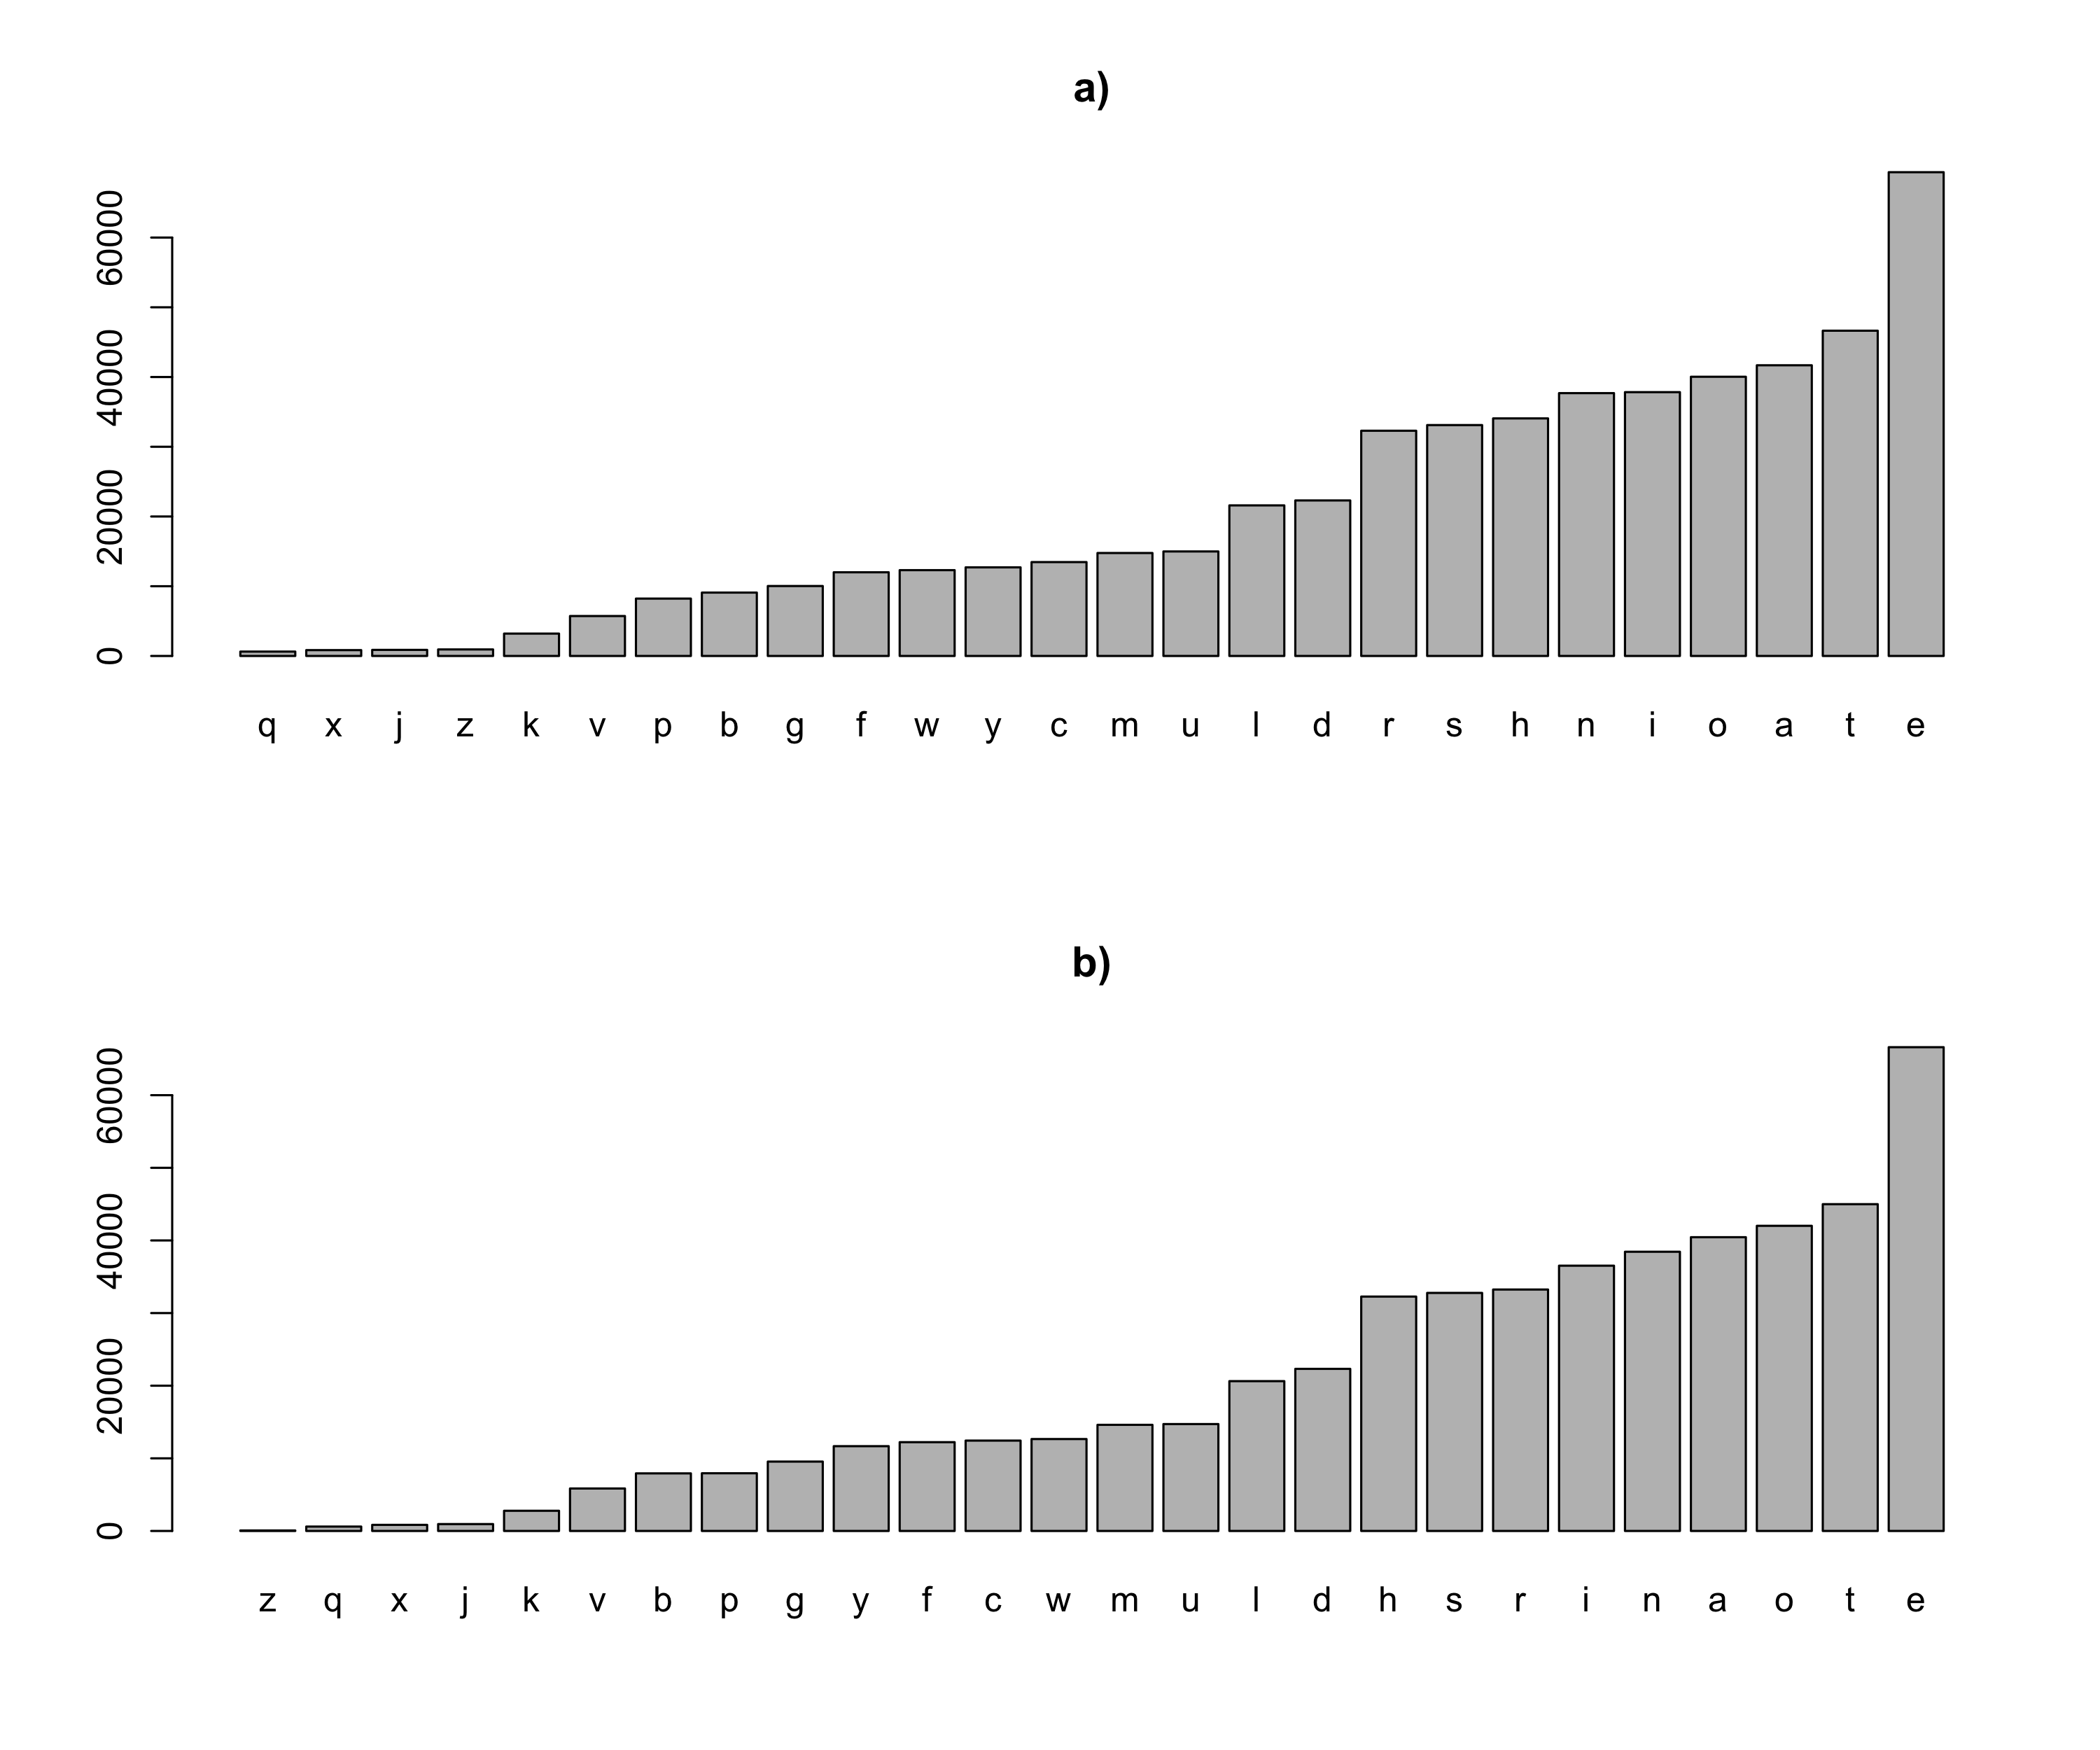
\includegraphics[width=\linewidth]{barplot52.png}
	\caption{Data exploration by letters of the book Pride and Prejudice (sub figure a)) and Sense and sensibility (sub figure b)) by Jane Austen.}\label{fig1}
\end{figure}

Using the library of \texttt{gutenbergr} we downloaded both books to different variables and with the help of other libraries such as \texttt{dplyr} and \texttt{tidytext} we organized some of its information. In the case of sub figure \ref{fig1} we started with the comparison of the most frequent letters. In both sub figures \ref{fig1}a) and \ref{fig1}b), we had to put a threshold of more than 10 on the frequency, because all of the occurrences bellow that were only numbers. We suspect that they represented the chapter numbers. In both books, the placement of the vocals on the frequency is almost identical, and there are only a few swaps of positions on the consonants. The reason of the similarity can be because both are written in English and are from the same author, so it tends to have similar forms of expression.\\

\begin{figure}[htp]
	\centering
	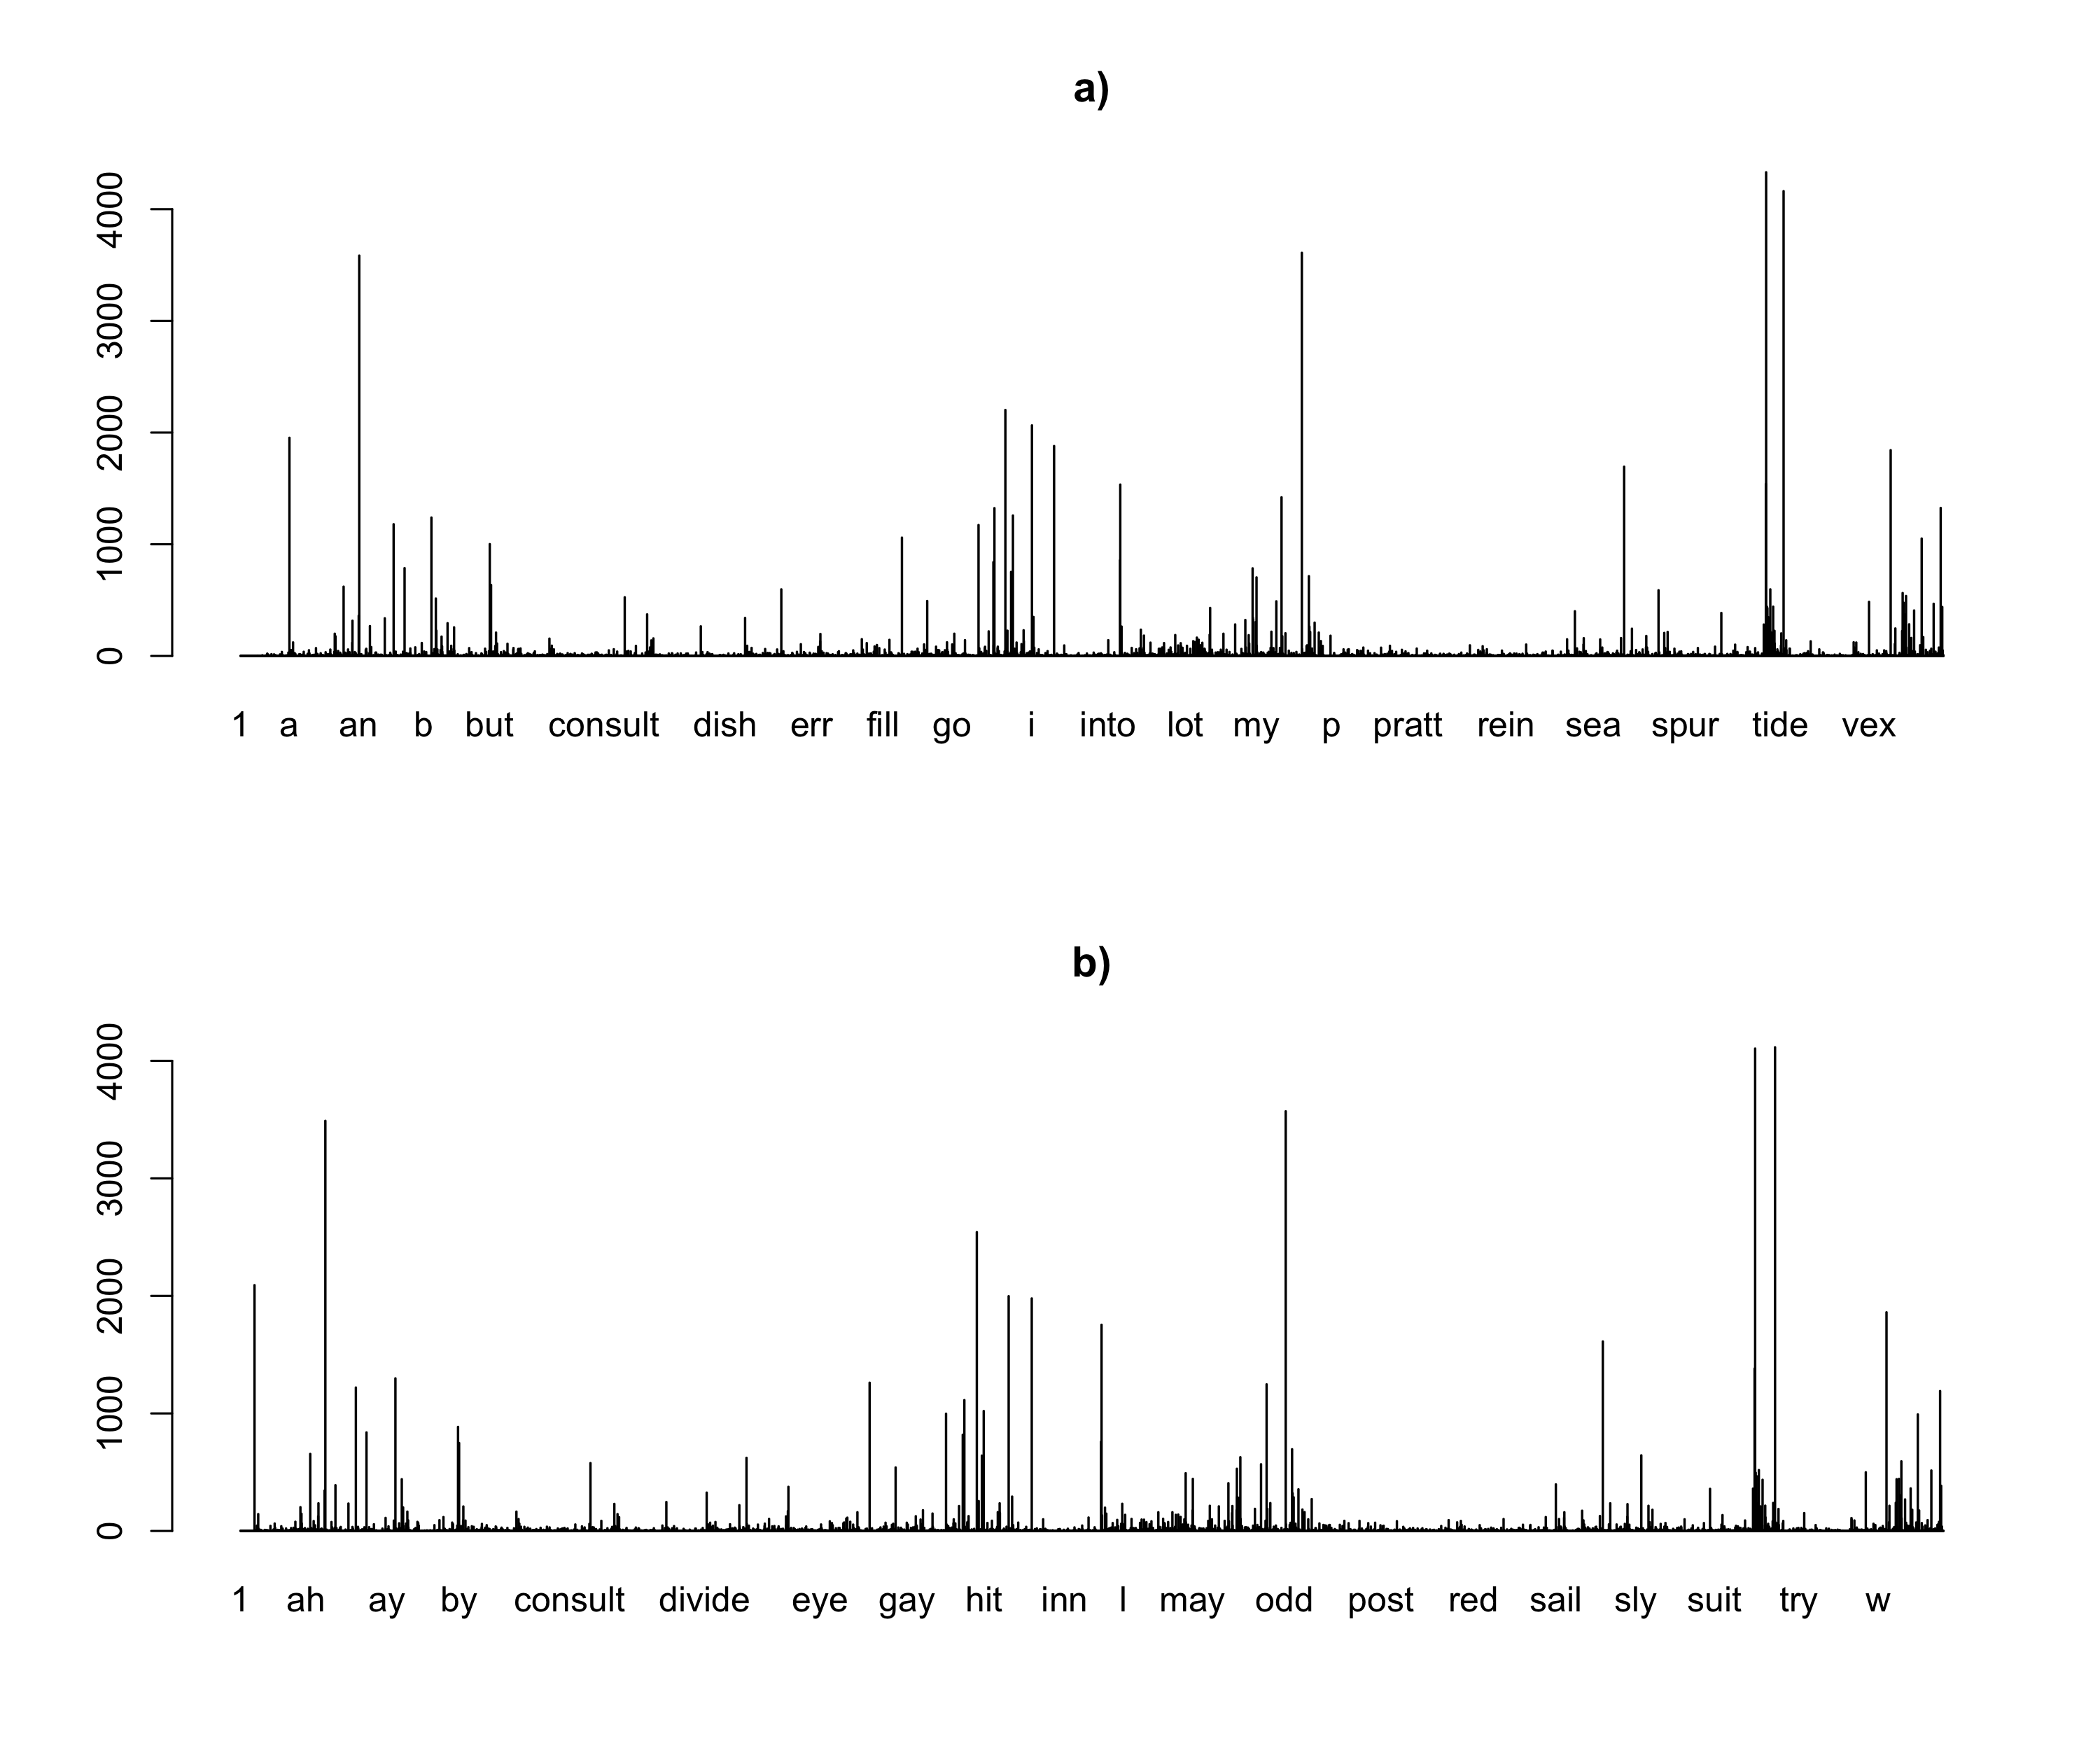
\includegraphics[width=\linewidth]{barplot51.png}
	\caption{Data exploration by words of the book Pride and Prejudice (sub figure a)) and Sense and sensibility (sub figure b)) by Jane Austen.}\label{fig2}
\end{figure}

We move on to see the frequency of the words. In this case, in figure \ref{fig2} we expected some similarities on the most frequent words but without giving extra instructions to order them and filter the ones with low frequency, it is not very clear the information that we can gather from this plot. \\

Something that jumped out while reviewing figure \ref{fig2} was that the sub figure \ref{fig2}b) had the word \textit{gay} in it. As mentioned before, both books are personal favorites, so it was a little strange that this word was here, because no character was described in that way on the Spanish version. So after some research we found out that the word \textit{gay} in the context of the 13th to 18th century meant something different than what it means in present day. Back then it meant happy or bright and lively looking. In a video made by PBS \cite{pbs} it exposes that the word \textit{gay} was later adopted as the meaning of same sex attraction because the other word to describe it, homosexual, was meant with a bad psychological connotation, and the word gay was a way to avoid the criminalization of same sex relationships.\\

In a not so serious article some people speculate that Jane Austen used this term deliberately, mainly because some of her social commentary on her books where often obscured, and also because by the time she published her books, the use of the word gay was slowly catching up to the general public. \\

\begin{figure}[htp]
	\centering
	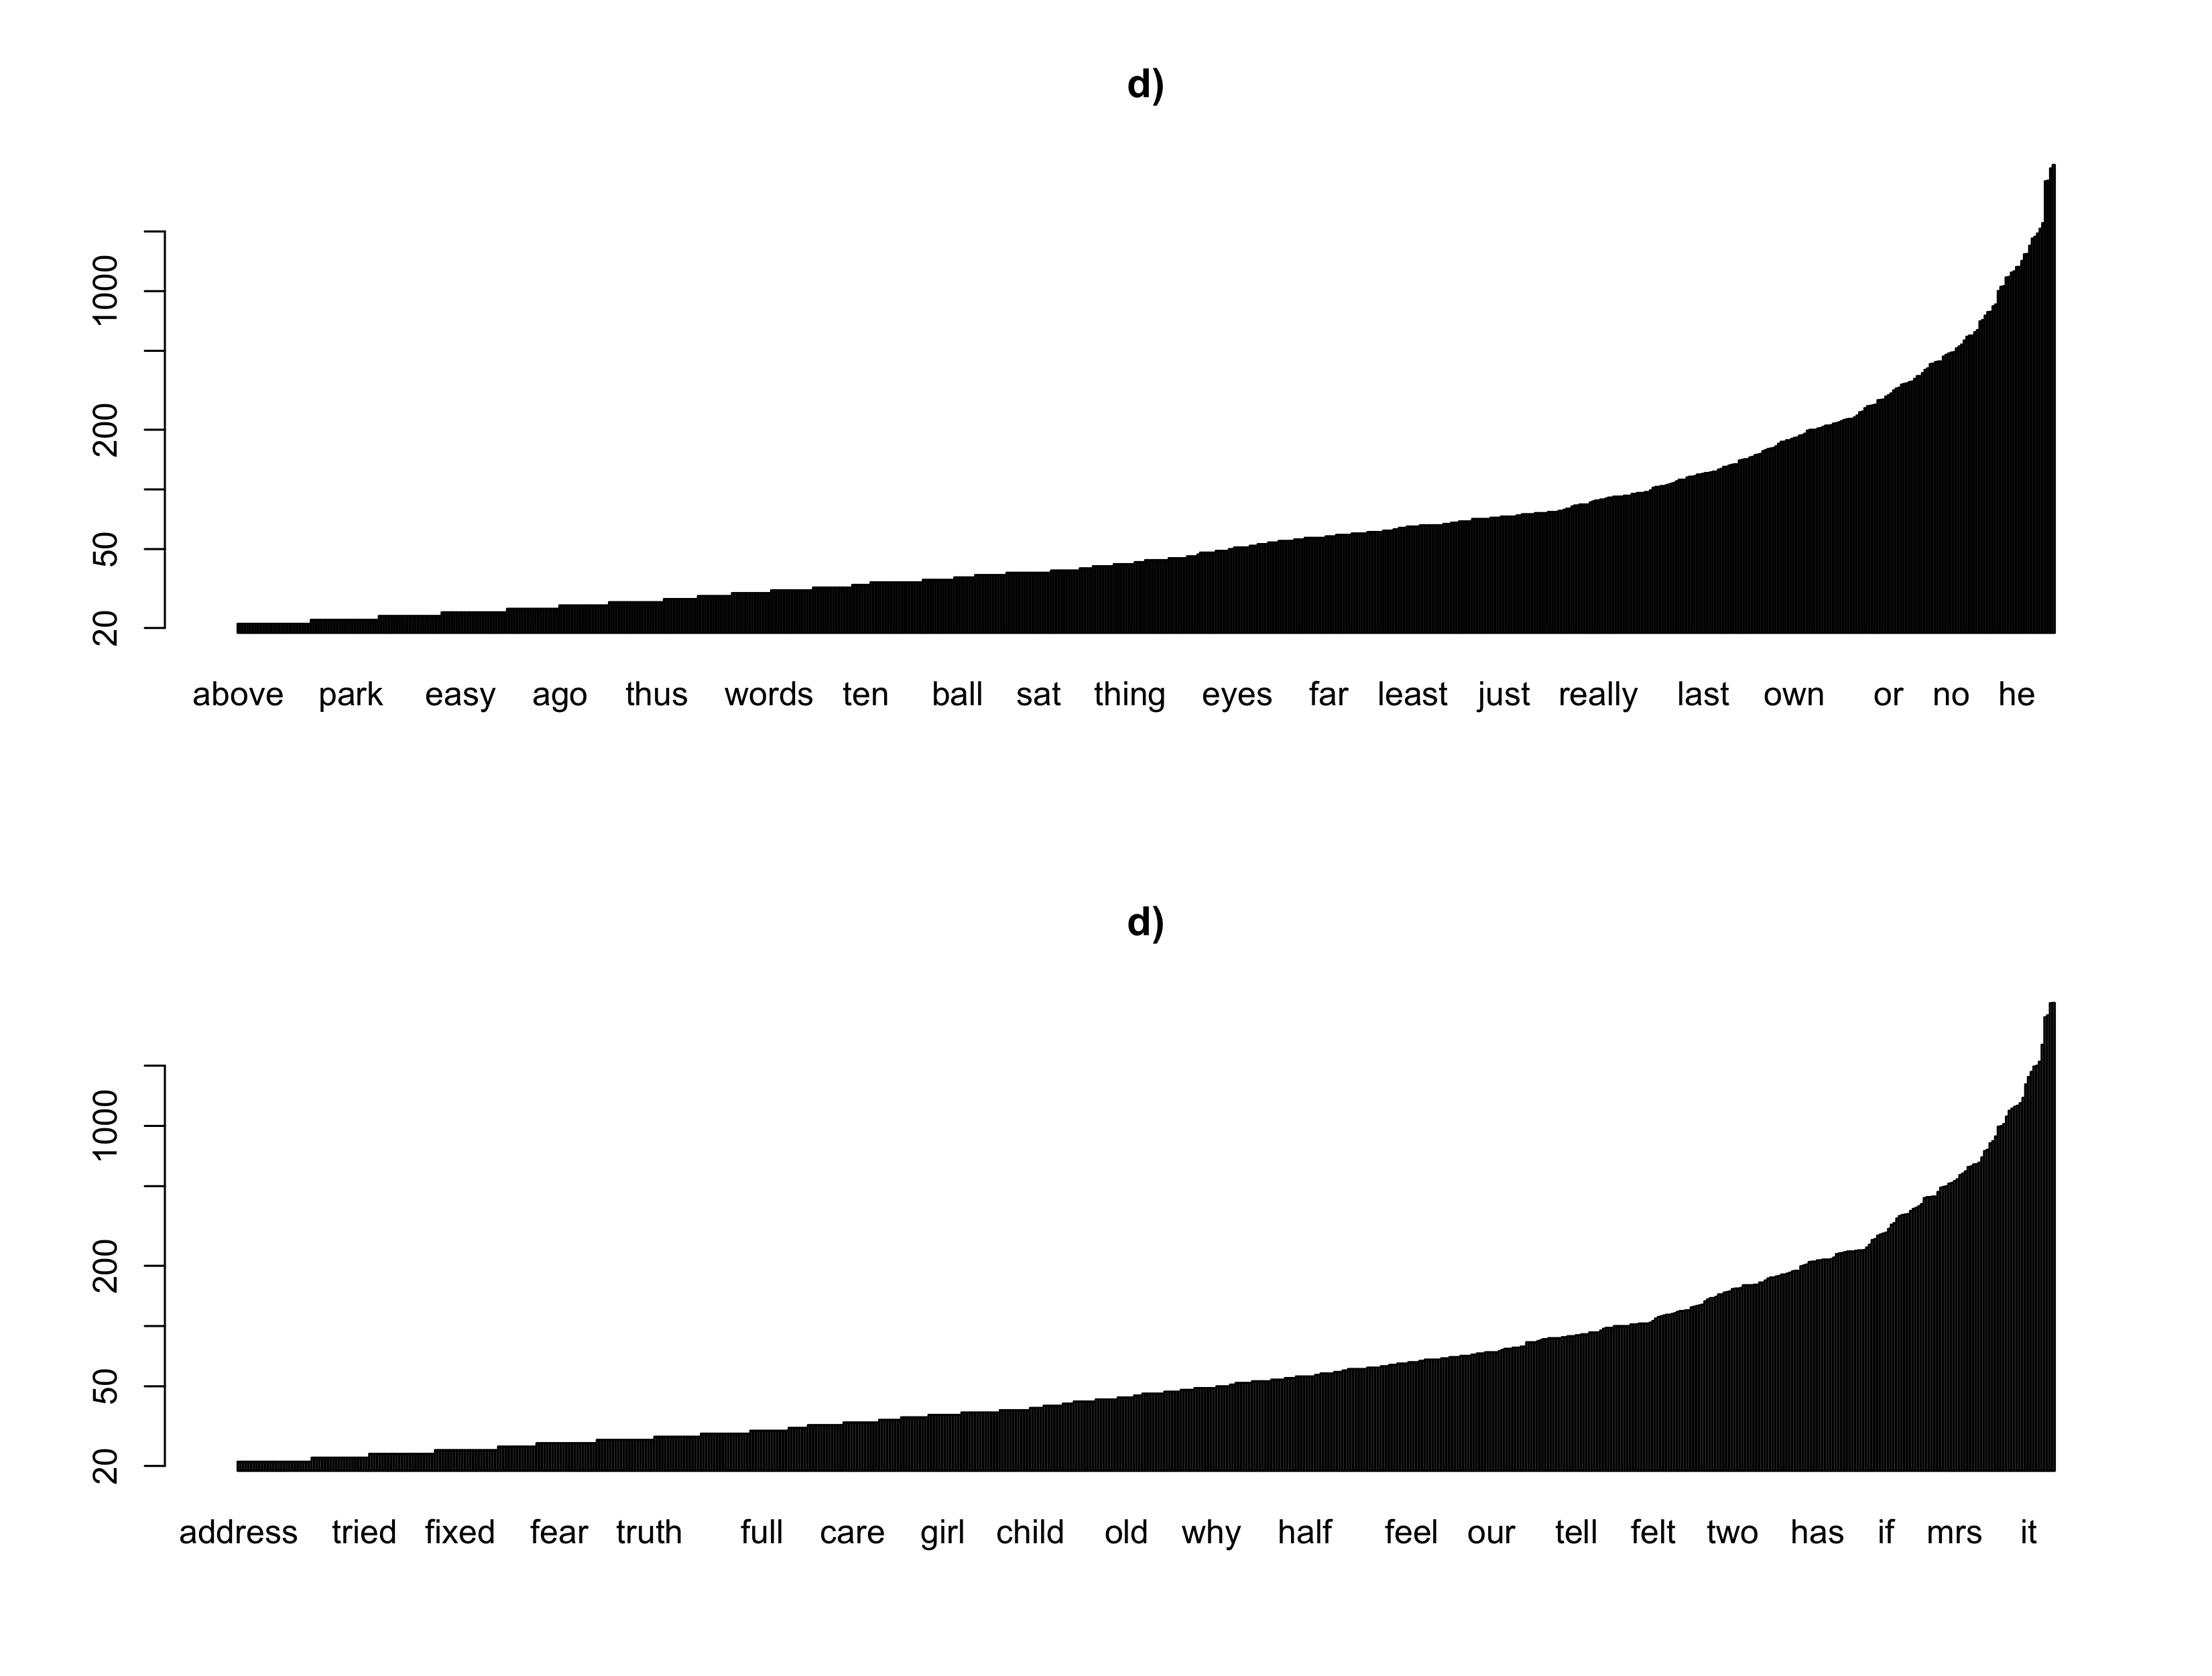
\includegraphics[width=\linewidth]{barplot53.png}
	\caption{Data exploration by words, ordering the data from lower to higher and filtering frequency to more than 20 occurrences. Pride and Prejudice (sub figure a)). Sense and sensibility (sub figure b))}\label{fig3}
\end{figure}

To be able to watch properly the distribution of the frequency on the words, we ordered them from lowest to highest number, taking out all the words with less than 20 recurrence in the data. Then, because the highest words where mostly connectors such as \say{the, a, as, for, by,} etc. we used the \texttt{log} value to even out the data, so it can be distinguishable. We can appreciate the results on figure \ref{fig3}.\\

 In sub figure \ref{fig3}a) there is a variety of words. For someone who has not read the book, it may be hard to make sense of it, but analysing the word, \textit{park} is interesting because almost a third of the books, we talk about great states that the main male characters have or are related somehow, for example, Rossings, Pemberly, Longbourn, Netherfield and Haye-Park (all of them fictional). The importance of the places are there to remained the reader that this are not only very wealthy man, but also how it will benefit our protagonists to end up with one of them. \\
 
 The word \textit{ball} also stands out, because, as our protagonist Elizabeth Bennet often states, the best way to meet people and encourage affection is by dancing with said partner. In the structure of the books, the balls take such importance, because each builds a big event for Elizabeth. Meeting Darcy for the first time. Being rejected by him in a rude manner. Getting close with Mr. Wickham. Each dance she forms different opinions on Darcy, that help her build a rather misguided opinion on his future husband.\\
 
 The word \textit{eyes} just sparkle joy, because one can assume is there because Darcy keeps talking about Elizabeth's eyes for half of the book.\\

As for sub figure \ref{fig3}b) there is a combination of words that immediately steers attention to the main plot. In this case, the combination of the words \textit{girl, child,} and \textit{truth} could be alluding to the scandal on Willoughby side of the plot, where he neglects to tell the sister's protagonist Marianne that he has an illegitimate child that he has not claimed, while he is courting her. This is a big part of the plot, that helps Marianne grow from 
idealistic romantic to a more mature young lady. \\

The other word that it is very interesting to see on this plot is \textit{old}, because one of the main reasons Marianne seems reluctant to accept the affections of Colonel Brandon is that he is 34, and she is 16. It can also allude to the fact that our protagonist Elinor is reaching an age in which it is deemed a bit old not to be married, and it is constantly reminded of that by Mrs Jennings.\\

\textit{Tired, fear}, and \textit{care} can also be attributed to the side of the plot in which the older half brother of the Dashwood sisters is often neglectful in taking care of them and his step mother, because of the poisonous advice of his wife, Fanny.\\

\section{Plot comparison}

This two books where chosen to be analysed because of its many similarities on their plot. In both cases we have a main protagonist that has only sisters, and is at the mercy of a good marriage to salvage the situation, that in that period was that a woman could not hold possessions, let that be money or state. In the case of Elizabeth, the absence of a brother leaves them at the mercy of their cousin, Mr Collins. And in Elinor case, they are dependent on their half brother, who resents his sisters because they were closer with his father. \\

They both have a favorite sister, Jane and Marianne respectively. And all of them have different good prospects for marriage that get complicated as the plot advances and their low social status gets in the way of forming a relationship.\\

Having established that, the next plots show the influence that the important characters have by measuring the frequency that they appear in the story. \\



\begin{figure}[htp]
	\centering
	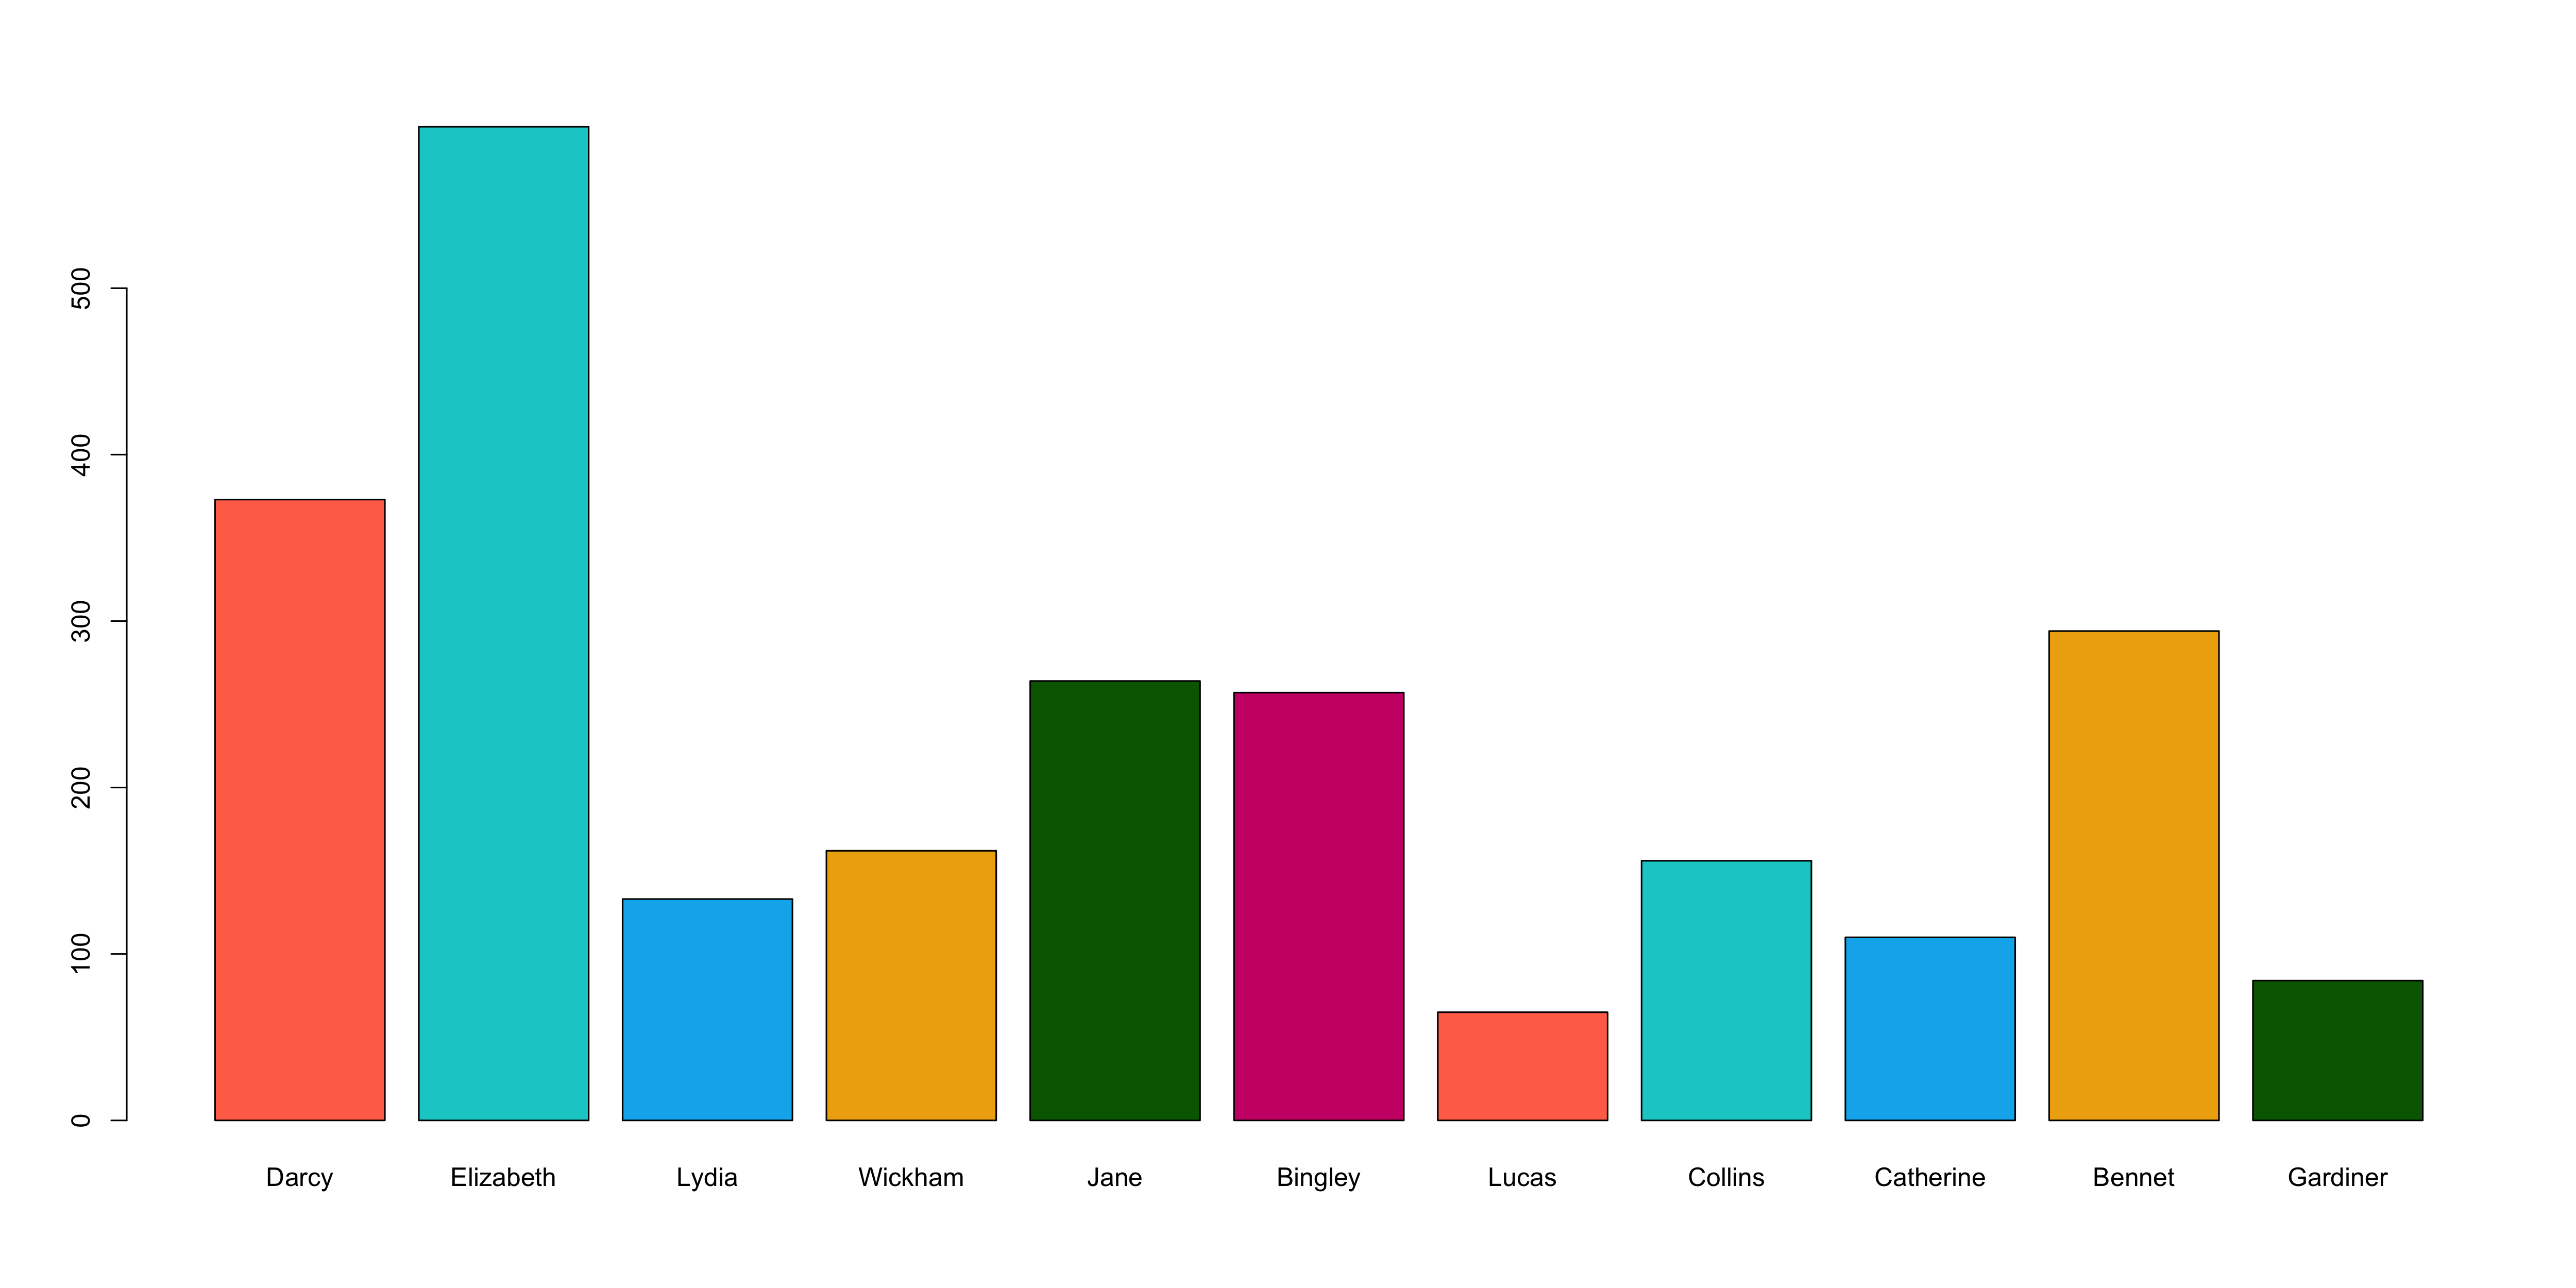
\includegraphics[width=\linewidth]{barplot_pp.png}
	\caption{Bar plot of the frequency of characters in the book Pride and prejudice}\label{fig4}
\end{figure}

In figure \ref{fig4} we quickly realize that Elizabeth is our main protagonist. Darcy is the main love interest, and Wickham is the secondary. Wickham represents one of the main reasons why Elizabeth and Darcy do not get together at first. As the story progresses his character gets known to be a liar and a cheat, but he ends up getting married to Elizabeth's younger sisters, Lydia by convincing them to run away. Jane is the favorite sister, and is cute that she gets mentioned almost the same amount as Bingley, which ends up being her husband. \\

Collins gets mentioned almost as much as Wickham, and that is curious, because he was also (in his mind) a contender for Elizabeth's affection. He tried to propose to her offering to save their family from destitution of their house, but Elizabeth rejected him.\\

Bennet is the last name of our protagonist, and in this case it gets mentioned so much, because there are 5 miss Bennet, a Mrs. Bennet and a Mr. Bennet. And they interact in the plot quite a lot. The Gardiners are the uncles of Elizabeth, and they are in the figure, because they helped a lot in all the problems the family encountered.\\

\begin{figure}[htp]
	\centering
	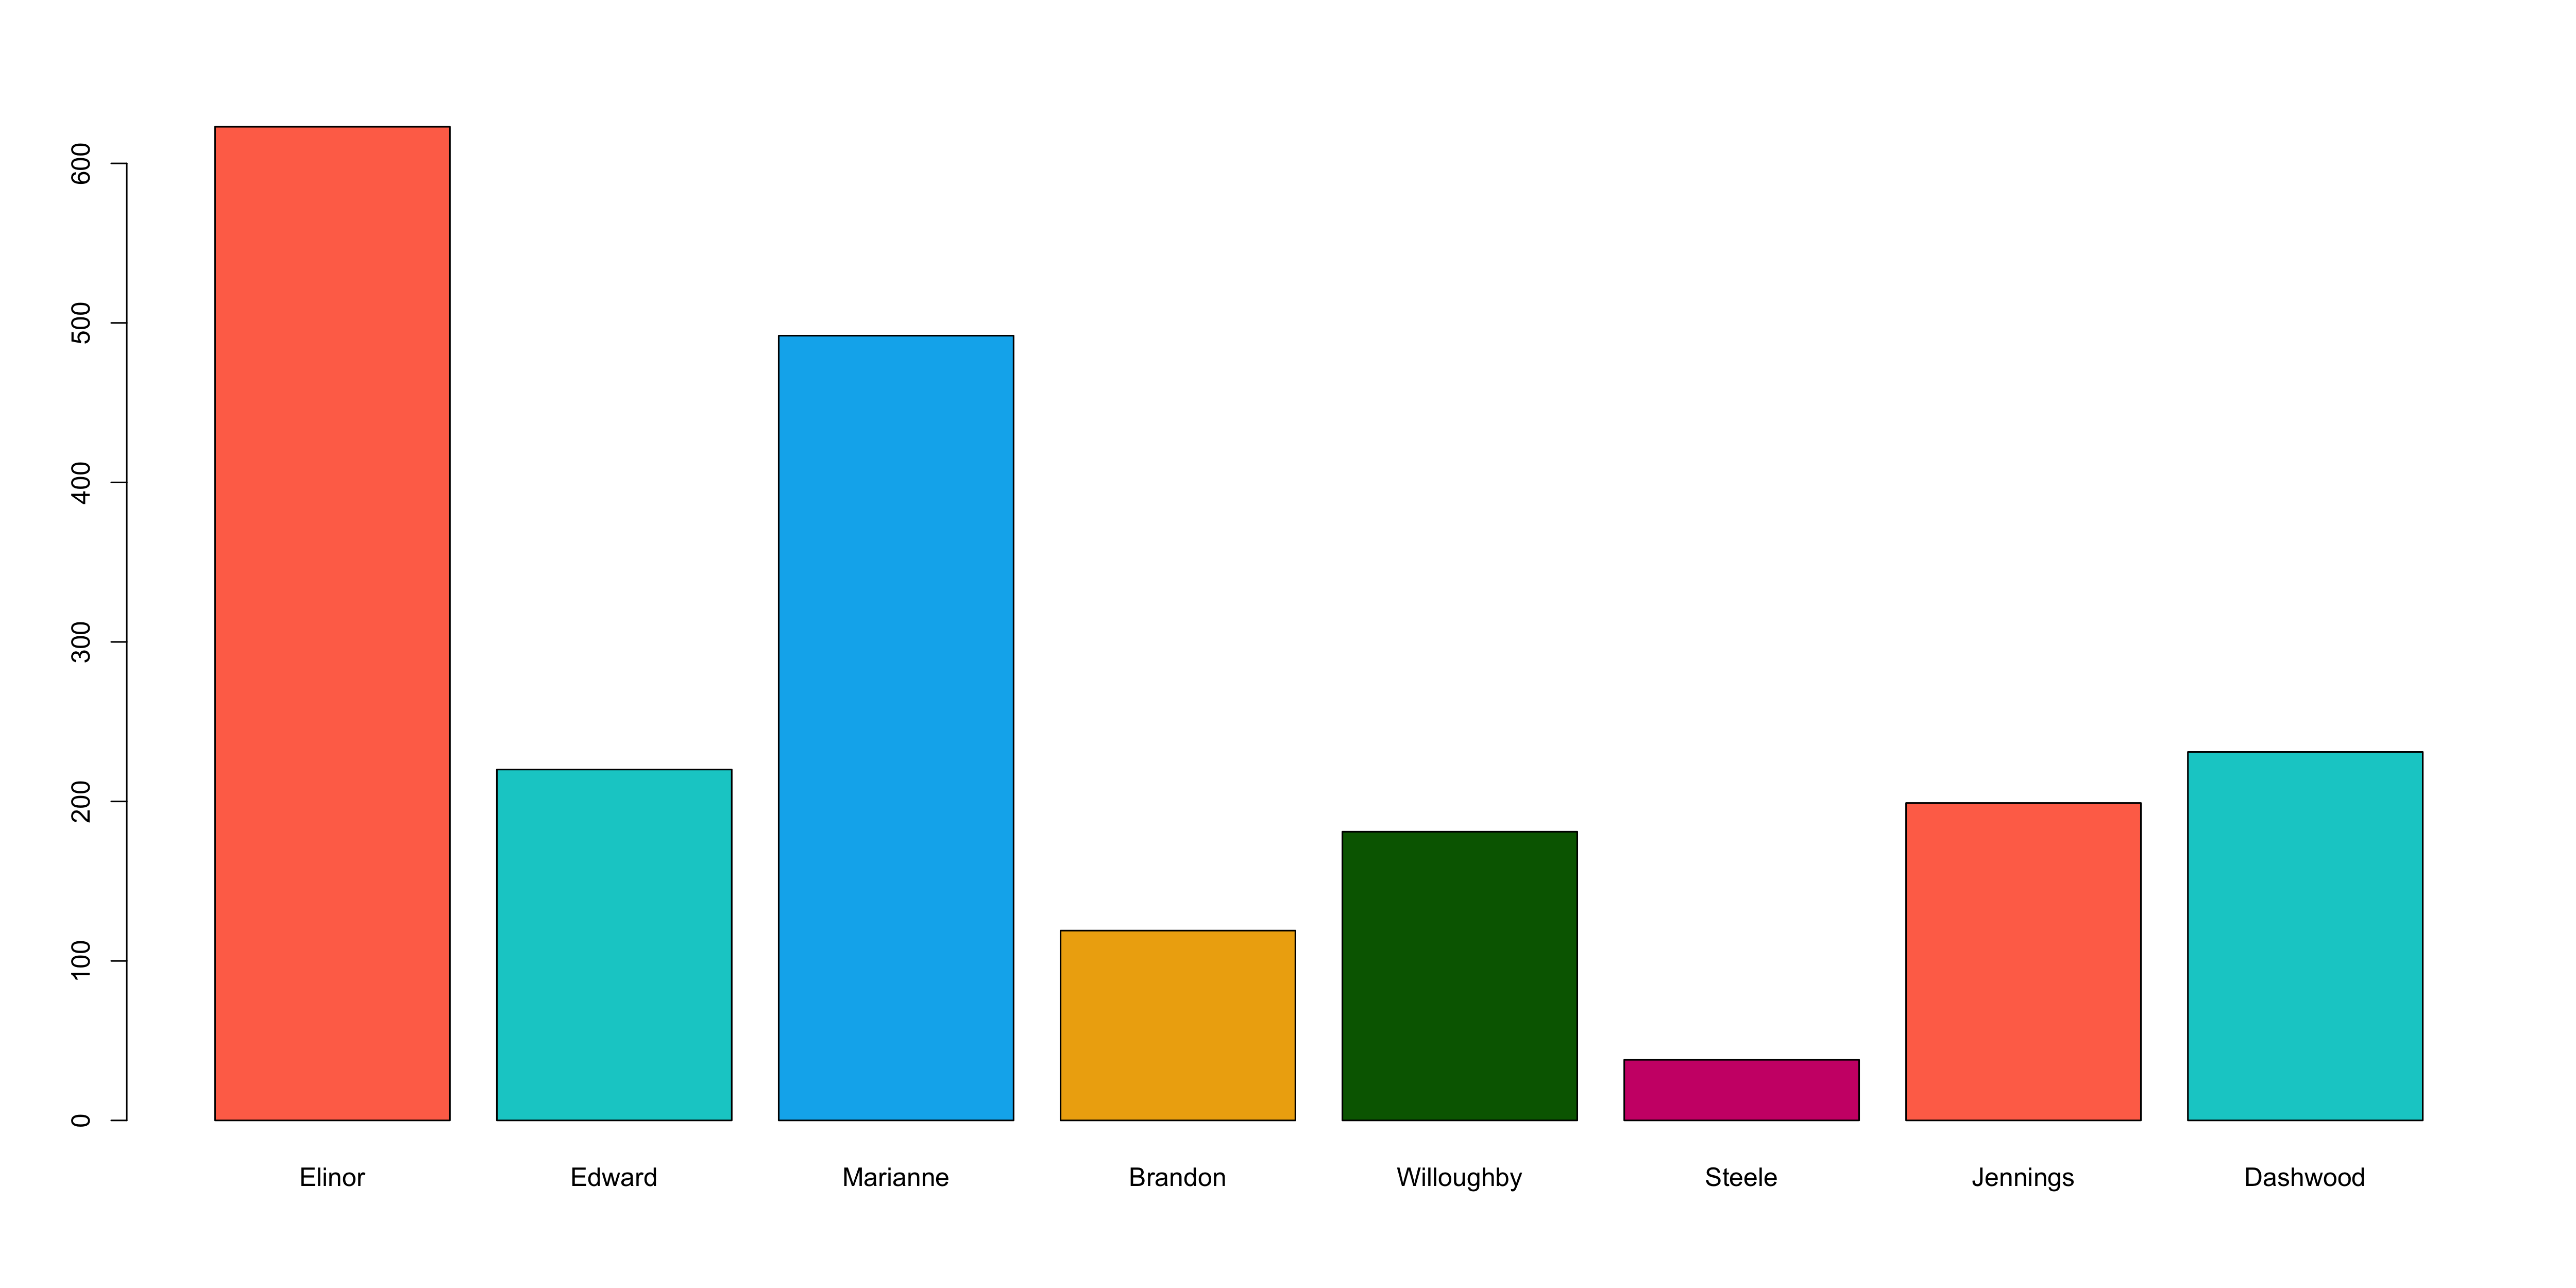
\includegraphics[width=\linewidth]{barplot_ss2.png}
	\caption{Bar plot of the frequency of characters in the book Sense and sensibility by Jane Austen.}\label{fig5}
\end{figure}

In figure \ref{fig5} we also see clearly that our protagonist is Elinor. But in this case, Marianne, her sister is almost as active in the plot as her. Whilst Elinor only has one love interest, Edward, Marianne has two. Colonel Brandon and Willoughby. It is quite sad that Brandon gets mentioned so much less than Willoughby since he is the one who ends up married to Marianne, but as we stated before, Marianne favored Willoughby up until the day he left her to marry some other richer girl. \\

Dashwood is the last name of our protagonists. And Jennings is the name of the meddler in the story. She tried her best to accommodate Marianne and Elinor with their respective partners, but always managed to make things worst.\\

\section{Other experiments}

As we played with the different variables and forms we could use the libraries in R, we created a variable with only the non repeated words of the story of Pride and prejudice. Just for fun, we tried to see how far in the story it stoped making sense without the repetition of the words. So here is the snippet: \\

\say{pride and prejudice by jane austen chapter 1 it	is a truth universally acknowledged that single man in possession of good fortune must be want wife however little known the feelings or views such may on his first	entering neighbourhood this so well fixed minds surrounding families he	considered rightful property some one other their daughters my	dear	mr bennet said	lady to him day	have	you heard	netherfield park let at last replied had not but returned she for mrs	long	has just been here told me all about made no answer do know who taken cried impatiently you tell i objection hearing was invitation enough why says young large from north england came down monday chaise four see place much delighted with agreed morris immediately take before michaelmas servants are	house end next week what name bingley married oh	sure	five thousand year fine thing our girls	 how can affect them tiresome am thinking marrying design settling nonsense} \\

Nonsense seemed like the right word to stop.\\

\section{Conclusions}

As a general conclusion, I had more fun with this practice that I thought I would have. Jane Austen is one of my favorite authors, and I really enjoyed getting a peek at what this plots would show me. In the end, I could have written so much more, because I love the plot of both books and the social commentary that the era reflects on marriage customs and the position of woman in society. It came as a surprise some of the information in the later plot, because of who ends up with who in the end. \\

Regarding the Gutenberg project, it was very interesting seeing all of those books available for download. Shakespeare, the Bronte sisters and Frankenstein have always been in my to read list, so now I could take a look at those works.\\




\bibliographystyle{plainnat}
\bibliography{tarea2.1}


 
\end{document}